In the present section, the steps that were taken in analysing the system to
develop are described. After the use cases and the necessary sensors are
determined, ythe system�s context could be bounded. At the end of the chapter,
the necessary algorithms will be presented with the help of activity diagrams.

The presented system analysis does not lay a claim on completeness but it
reflects all the standardised methods of analysing a system that were estimated
helpful in order to develop the system.

\section{Use Case Diagram}

Based on the requirements that were agreed on with the customer, two main use
cases of the system can be found:

\begin{itemize}
\item{Drive out of a perpendicular Parking Lot}
\item{Drive out of a parallel Parking Lot}
\end{itemize}

Both use cases have in common that at the end of the successful process, the
user has to regain the control over its vehicle in a defined way. Additionally,
the user should always have the possibility to interrupt the process and regain
the control over the car, even if the process has not yet finished. Each of the
use cases are triggered by the driver as well as they are supported by various
sensors and control systems.

\begin{figure}
\centering
\captionsetup{justification=centering}
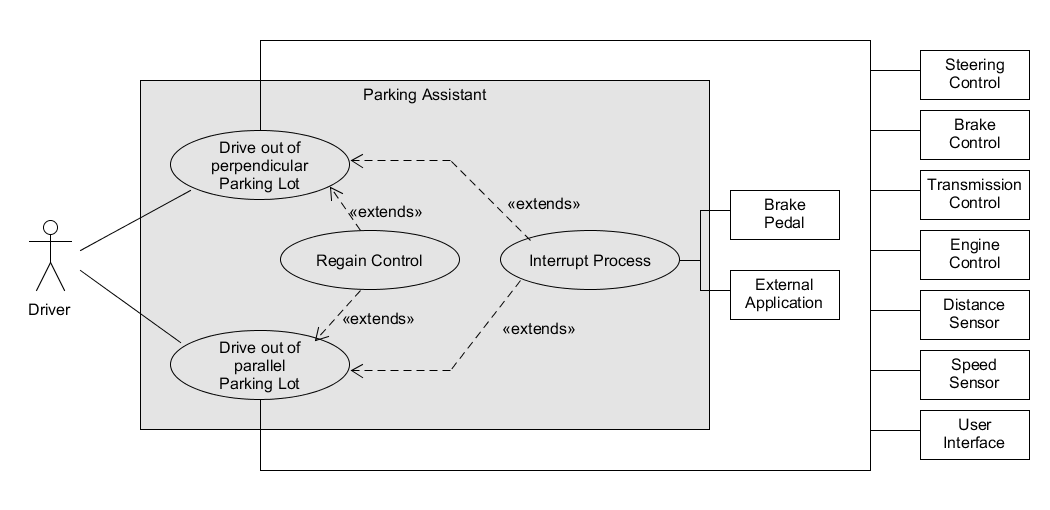
\includegraphics[width=\textwidth]{res/systemAnalysis/UseCase.png}
\caption{Overview of the System's Use Cases}
\label{fig:UseCases}
\end{figure}

\section{Sensor Overview}
\label{sect:sensors}
To support the presented use cases, the system needs an overview of the cars
surrounding. Six sensors, two of them cameras and 4 of them distance sensors,
are placed in the car to provide this overview. The placement of the sensors can be
retrieved from figure \ref{fig:SensorOverview}.

The sensors that are placed in the middle of the car�s front and rear are
cameras. In many cases cameras are already integrated in the car and provide the
user a realistic image of its surrounding. The distance sensors at the corners
of the bumpers might be radar- or ultrasonic-sensors. Radar sensors have the
advantage, that they might be placed within the bumper and that they are
therefore not visible.

\begin{figure}
\centering
\captionsetup{justification=centering}
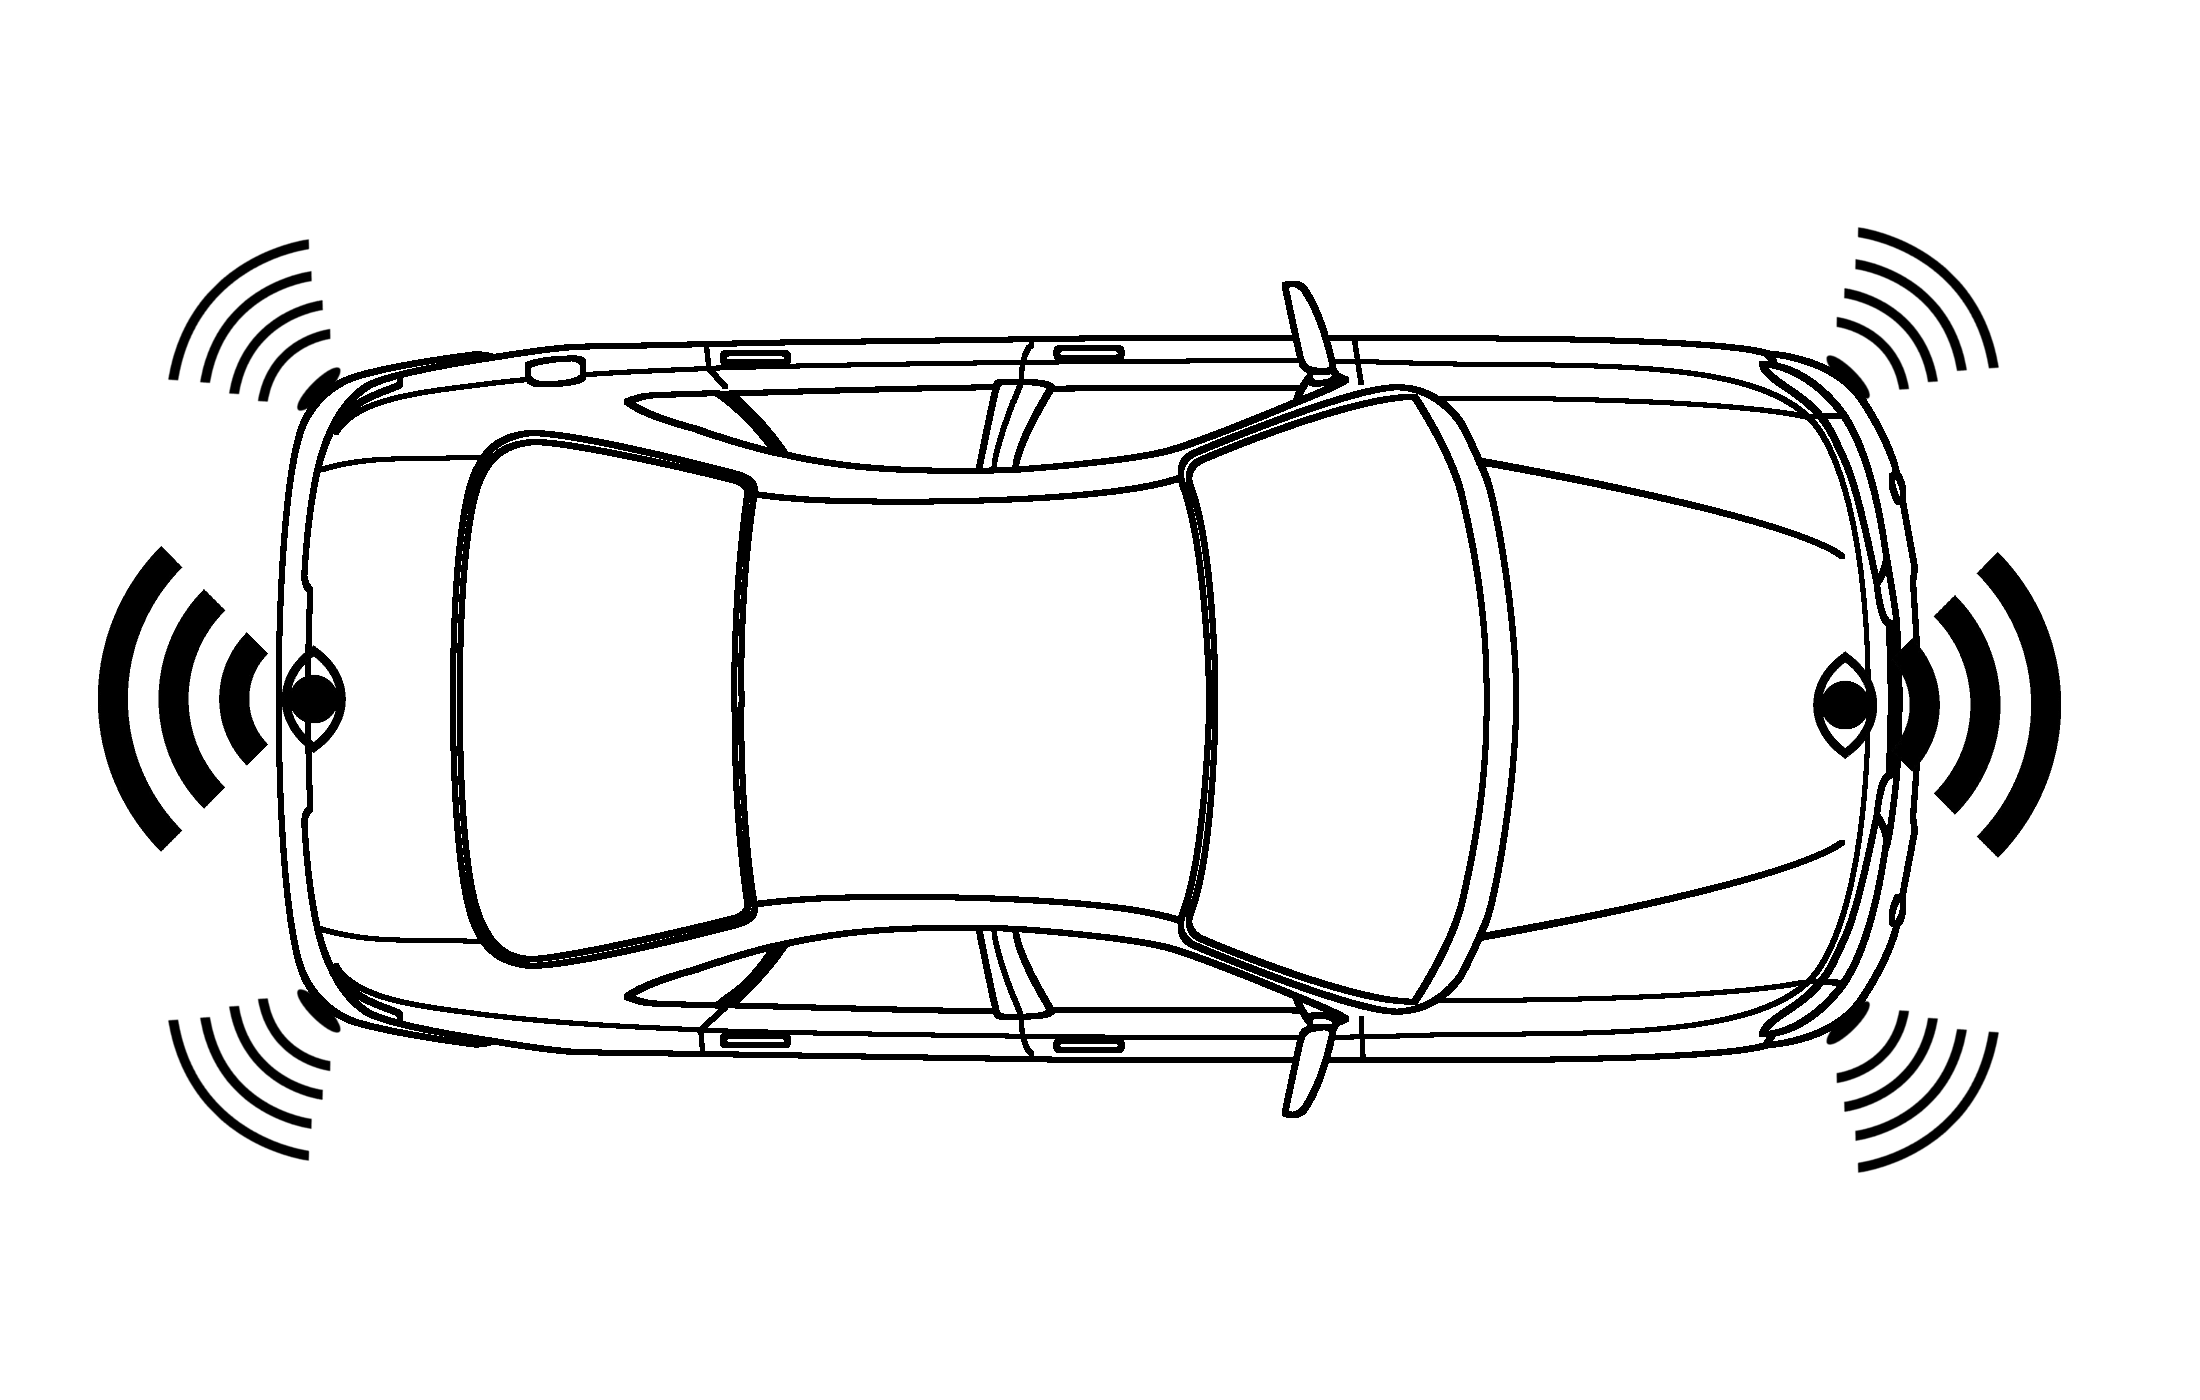
\includegraphics[width=0.75\textwidth]{res/systemAnalysis/SensorOverview.png}
\caption{Overview of the System' Sensors}
\label{fig:SensorOverview}
\end{figure}

\section{Context Diagram}

After the use cases and the required sensors have been found, the context of the
system to develop can be determined (see figure \ref{fig:ContextDiagram}).
Dataflows are depicted with solid arrows while signals that are used to control
the systems are sketched with dashed arrows.

Beside the sensor information, the graphical representation of the process and
the information that is sent to the car�s control systems, there exist two
systems that are used to interrupt the process of leaving a parking lot. If a
driver sits in the car and presses the break pedal, the process will be
interrupted immediately and the driver will regain the control over its vehicle.
If the whole process is controlled remotely without the driver sitting in its
car, the external application that controls the process should act as a dead
man�s switch that is operated by the user. If the signal from this application
is no more retrieved by the system, the process should be interrupted.


\begin{figure}
\centering
\captionsetup{justification=centering}
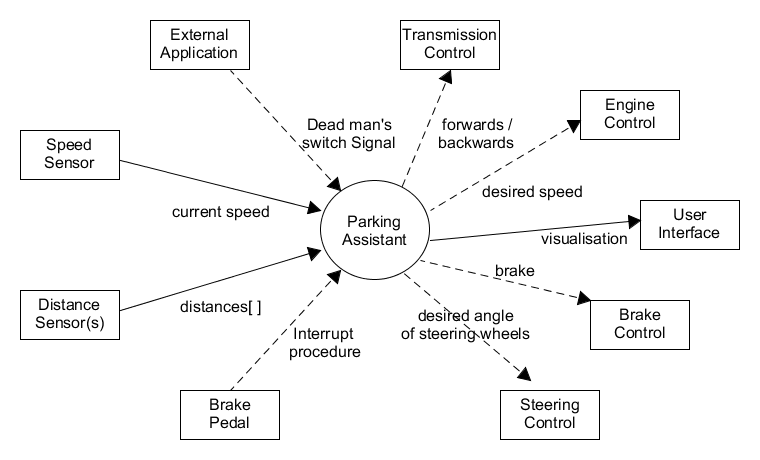
\includegraphics[width=\textwidth]{res/systemAnalysis/ContextDiagram.png}
\caption{Context Diagram of the System}
\label{fig:ContextDiagram}
\end{figure}

\section{Activity Diagrams}
After the previous sections presented the use cases as well as the involved
sensors and actuators, the current section presents the progress of leaving from
a perpendicular and a parallel parking situation. This presentation is done with
the help of activity diagrams that reflect the algorithm that has to be
implemented. Activity diagrams visualise the dynamics and the behaviour of a
system and therefore serve for a better understanding of the process.


\subsection{Activity Diagram Reverse Perpendicular Parking}
When leaving a perpendicular parking situation, there exist different cases
affecting the process that have to be analysed. This cases might impede the
system from successfully performing its action. Additionally, there are
different starting situations a car might be in before starting the process of
leaving a parking space. To analyse these cases and to develop an algorithm that
is able to deal with the possible cases and starting situations, the Best- as
well as the Worst-Case for the system are described.  The activity diagram of
the whole process can be seen in figure \ref{fig:ActivityPerpendicular}.

\begin{figure}
\centering
\captionsetup{justification=centering}
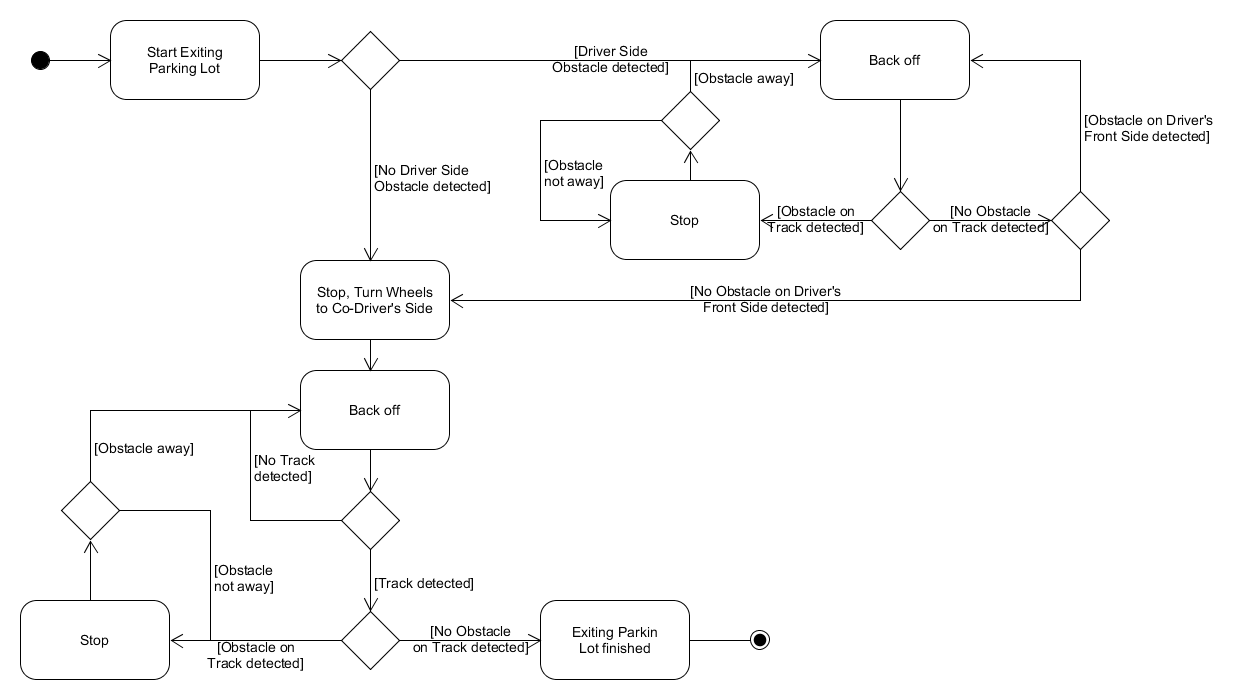
\includegraphics[width=\textwidth]{res/systemAnalysis/ActivityObstacleTransversal.png}
\caption{Algorithm for leaving a perpendicular Parking Situation}
\label{fig:ActivityPerpendicular}
\end{figure}

\subsubsection{Best Case}
The initial situation of the best case is the situation of there being no
obstacle on the driver�s side. The presence or absence of an obstacle is
determined with the help of the car�s sensors that have been introduced in
section \ref{sect:sensors}.

If there is no obstacle on the driver�s side, the car is able to turn its wheels
in the needed direction and start to drive backwards. For the case of leaving a
reverse perpendicular parking situation it is of no importance if there is an
obstacle on the passenger side because this won�t affect the process of leaving
the parking space.

The car now drives backwards till the moment it recognizes the roadway with the
help of the built-in camera. Additionally, the roadway is scanned for moving
obstacles like other cars, bicycles or persons during the whole process. If such
an obstacle is detected, the car stops and waits for the moving obstacle to
leave the safety-critical area. If there is no obstacle, if the detected
obstacle has disappeared of it has stopped approaching the car, the process can
be resumed and be completed.


\subsubsection{Worst Case}
In opposition to the previously described initial situation, the worst case is
given if there is an obstacle on the driver�s side. The process then changes in
a way that the car has firstly to drive back some distance before it can turn
its wheels safely without the risk of there being a crash with the detected
obstacle.

In the same way as it was described for the best case, the car scans its
surroundings while driving backwards if there are moving obstacles. In the case
of there being none of the possible obstacles, the car drives back until the
obstacle on the driver�s side is no more critical to the process and the car is
able to safely turn its wheels. The process that follows is now identical to the
previously described best case.

\subsection{Activity Diagram Parallel Parking}
Leaving a parallel parking situation also includes different initial situations
that have to be reflected. Analogously to the process of reverse perpendicular
parking, the best- and the worst case are described within this section. The
activity diagram of the whole process can be retrieved from figure
\ref{fig:ActivityParallel}.

\begin{figure}
\captionsetup{justification=centering}
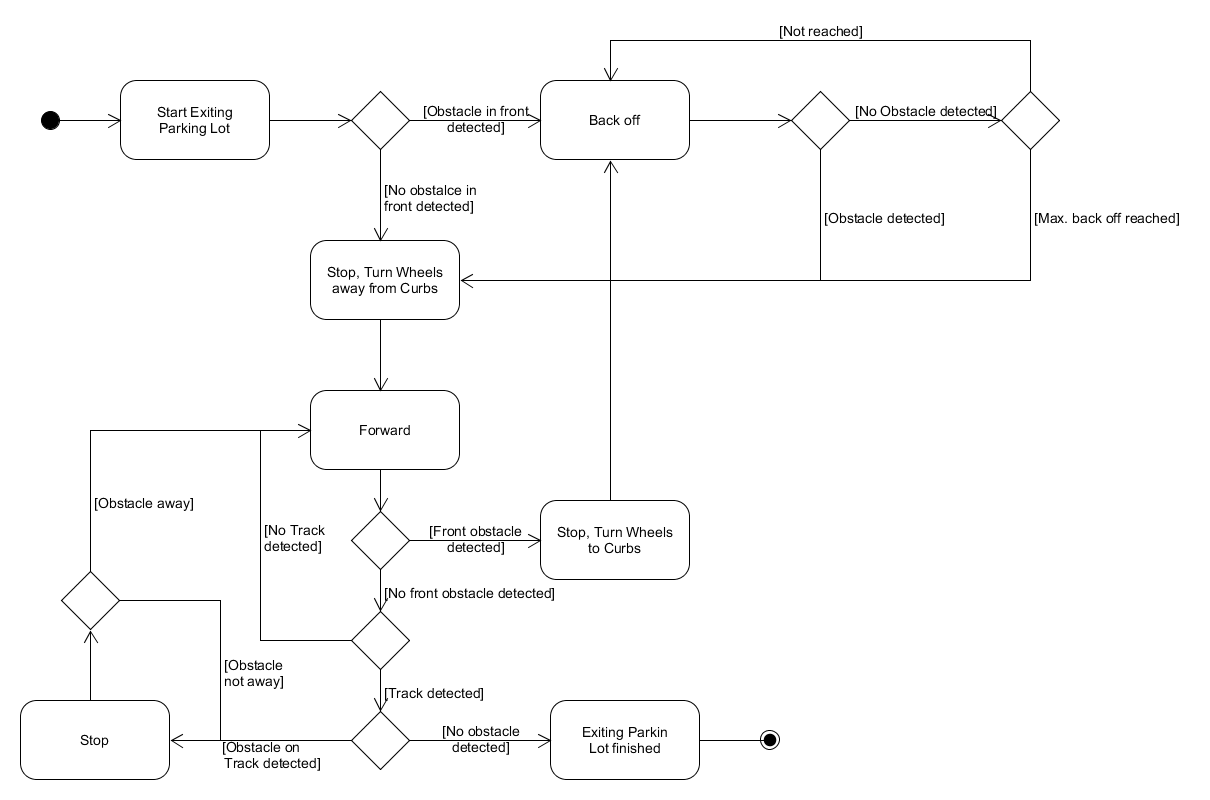
\includegraphics[width=\textwidth]{res/systemAnalysis/ActivityObstacleLenghtwise.png}
\caption{Algorithm for leaving a parallel Parking Situation}
\label{fig:ActivityParallel}
\end{figure}

\subsubsection{Best Case}
The best case in the current scenario is given if there is no obstacle in front
of the car that should be brought out from a parallel parking situation. In this
case, the car is able to turn its wheels towards the road side and to drive
forward safely. During the process of driving forwards, the system continuously
checks if there are either obstacles occurring in front of it or approaching
from the roadside. If an obstacle is detected, the process is again stopped and
only resumed if the detected obstacles have disappeared or if they do not
approach anymore.

\subsubsection{Worst Case}
The worst case is characterised by there being an obstacle both in front and
behind the car that should be brought out of the parking lot. The car then
starts to drive slowly backwards until it has reached the minimum safety
distance to the obstacle behind it. The wheels are then turned towards the
roadside and the car starts to drive forwards.

In the case that the car then detects an obstacle in front of it, it stops,
turns its wheels towards the curbs and starts to drive backwards. It continues
with its motion till it reaches the minimum safety distance either to the rear
obstacle or to the curbs. The car then turns it wheels to the roadside again and
drives forwards. These steps are repeated until the car is able to leave the
parallel parking situation and detects the roadway. Within the whole process,
the car�s surroundings are again checked for steady and for moving obstacles
respectively.

\section{Design Sketches}

A first design sketch has been developed (see figure \ref{fig:initialMockup})
and the customer�s feedback on the design has been gathered, this feedback is
used to create refined mockups. Since the customer requests two designs -- one
for the day and one for the night-mode -- two of these refined designs are
developed.

These newly designed mockups also take the customer�s feedback into account that
some outputs should be simplified and that the area where the sensor information
is presented should not be reduced. Instead, the area presenting the aerial view
is reduced and the sensor information are presented in a wider area.

\begin{figure}
\centering
\captionsetup{justification=centering}
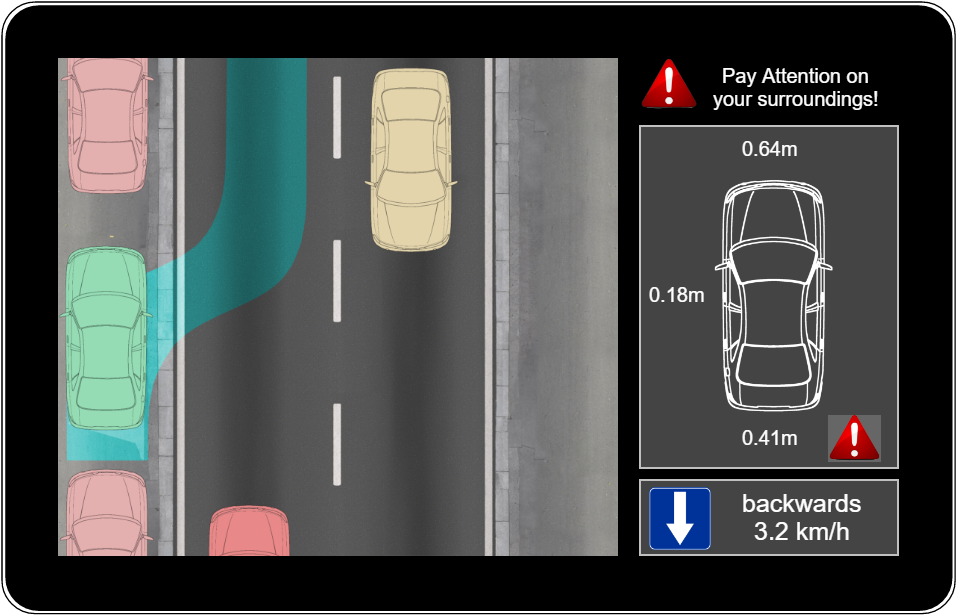
\includegraphics[width=0.75\textwidth]{res/systemAnalysis/darkskin.png}
\caption{Dark Skin of the final Design Sketch}
\label{fig:darkskin}
\end{figure}

\begin{figure}
\centering
\captionsetup{justification=centering}
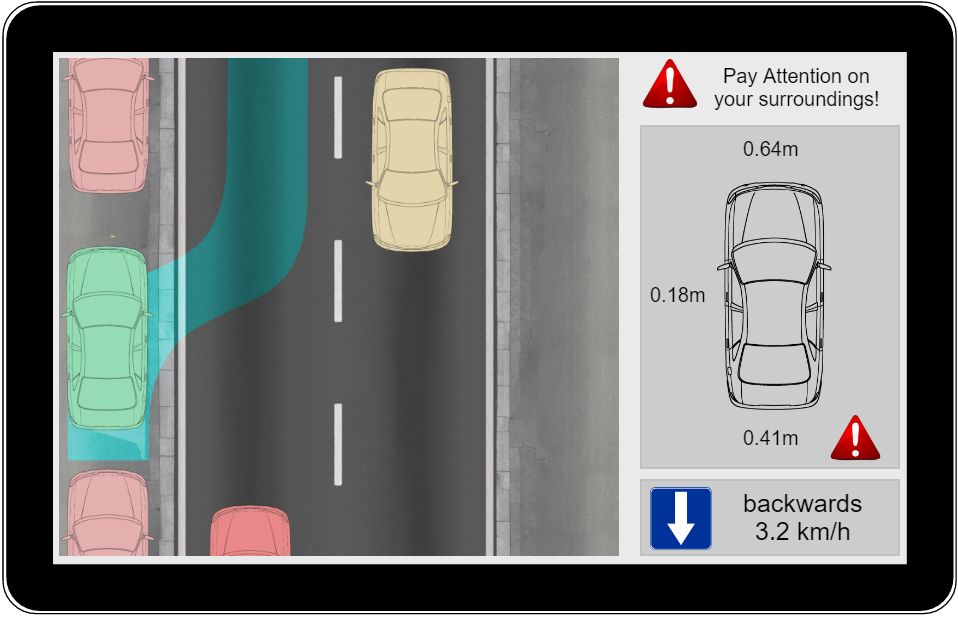
\includegraphics[width=0.75\textwidth]{res/systemAnalysis/brightskin.png}
\caption{Bright Skin of the final Design Sketch}
\label{fig:brightskin}
\end{figure}
